\chapter{Chatbot}
\section{Legal Consultation Process and Development Challenges}
Legal consultation for gender-based cases involves a complex interplay of factual assessment, 
legal analysis, and interpersonal support. To understand the challenges our agentic pipeline 
aims to address, it is essential to examine the current process of legal consultation in the 
Colombian context, particularly within institutions like the Consultorio Jurídico de la Universidad de los Andes.

When conducting initial consultations, legal experts engage in a structured yet flexible 
information-gathering process. This typically begins with open-ended questions about the 
client's situation, followed by increasingly specific inquiries to establish relevant facts, 
timelines, and supporting documentation. Throughout this process, legal practitioners must 
balance multiple objectives: identifying legally relevant details, establishing case chronology, 
determining applicable legal frameworks, assessing procedural options, and evaluating evidentiary 
strengths and weaknesses.

In the specific context of gender-based cases, this process becomes particularly nuanced. 
Legal experts must navigate sensitive topics such as domestic violence, sexual harassment, 
discrimination, and family conflicts while maintaining professional boundaries and creating 
a safe environment for disclosure. The consultation process often requires practitioners to 
recognize both explicit and implicit elements of gender-based issues, including power dynamics, 
economic dependencies, and potential safety concerns that may not be immediately articulated by clients.

At the Consultorio Jurídico de la Universidad de los Andes, consultations serve a dual purpose. 
Beyond providing legal guidance, practitioners offer crucial emotional support to clients navigating 
traumatic or stressful situations. This holistic approach recognizes that legal challenges do 
not exist in isolation from psychological and social contexts. Practitioners are trained to 
acknowledge emotional aspects of cases while guiding clients toward practical legal 
solutions—a balance that any automated system must similarly attempt to achieve.

The Consultorio Jurídico operates as a social service initiative, providing free legal assistance 
to populations that cannot afford private legal representation. This service, typically costly 
in the commercial sector, forms part of the university's commitment to social responsibility 
and access to justice. Law students, supervised by experienced attorneys, gain practical 
experience while serving vulnerable communities, creating a mutual benefit model that contributes 
to both legal education and social equity.

A significant challenge in developing technological support for this process is data access. 
The Consultorio Jurídico maintains detailed records of consultations, including case notes, 
legal analyses, and outcomes. However, these records contain sensitive personal information 
and are not anonymized, making them unsuitable for sharing with third-party researchers or 
technology developers. Client confidentiality and ethical considerations rightfully prevent 
direct use of these authentic case records for AI development purposes.

This data limitation creates a methodological challenge for our research. Without access to 
real consultation transcripts or case files, we must develop alternative approaches to creating 
representative datasets for training and evaluating our agentic pipeline. This necessitates 
collaboration with legal experts to generate synthetic cases that reflect the patterns, 
complexities, and legal issues commonly encountered in gender-based consultations, while ensuring 
no actual client information is compromised.
Additionally, the consultation process varies significantly based on the specific legal issues 
involved. A domestic violence consultation may focus heavily on immediate protective 
measures and evidence documentation, while a workplace discrimination case might center on 
establishing patterns of differential treatment and identifying appropriate administrative and 
judicial remedies. This diversity of case types requires any automated system to be flexible enough 
to adapt its information-gathering approach based on the emerging understanding of the case category.
The temporal dimension of legal consultations also presents challenges for automation. 

Initial consultations often reveal only partial information, with critical details emerging over 
subsequent interactions as trust is established and clients recall or discover relevant information. 
This iterative process must be accommodated in any agentic system, allowing for recursive 
information gathering and strategy refinement as case understanding evolves.
Finally, the legal consultation process culminates in strategy formation—identifying viable 
legal pathways, explaining procedural requirements, outlining potential challenges, and setting 
realistic expectations about timelines and outcomes. 

This guidance must consider not just what is legally possible 
but what is realistically achievable given the client's resources, priorities, and circumstances. Our system must not only extract relevant information and provide legal guidance but must do so in a manner that acknowledges the emotional 
and practical dimensions of gender-based legal challenges in the Colombian context.

\section{Dataset Construction}
\label{sec:dataset}

Our dataset development followed an iterative human-AI collaboration process comprising four key phases, 
as illustrated in Figure~\ref{fig:legal_data}.

\begin{figure}[htbp]
    \centering
    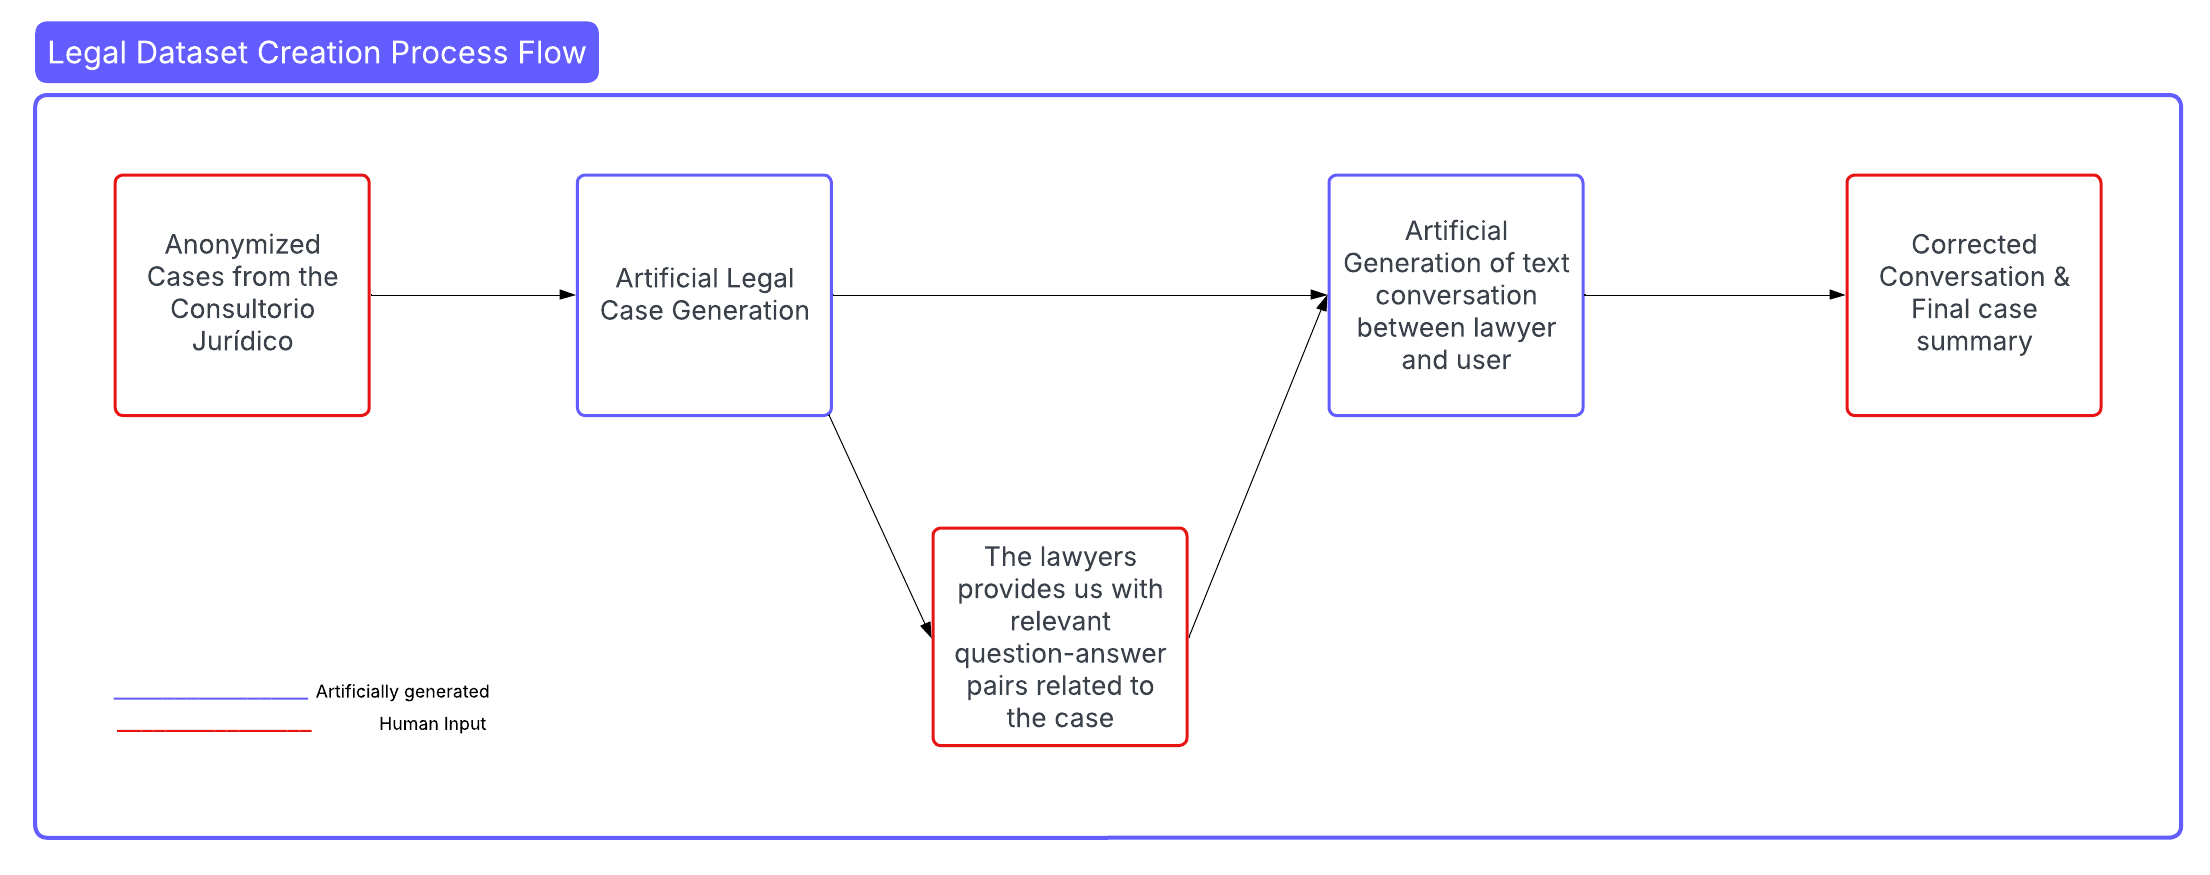
\includegraphics[width=0.7\textwidth]{figures/Legal_dataset.png}
    \caption{Legal Dataset Creation}
    \label{fig:legal_data}
\end{figure}

These phases are Synthetic Case Generation, Expert-Guided Refinement, Conversation simulation and Legal Strategy Development.

\subsection{Base Case Preparation}
The initial phase focused on establishing a foundation of real cases while ensuring privacy of the parties involved:
\begin{itemize}
    \item Initialized with 23 anonymized gender-based case summaries from the Consultorio Jurídico
    \item Categorized cases into primary themes including:
    \begin{itemize}
        \item Violencia Basada en Género
        \item Derechos Sexuales y Reproductivo
        \item Violencia Económica
        \item Violencia Sexual
        \item Violencia en el Ámbito Familiar
        \item Violencia en el Ámbito Laboral
        \item Violencia Institucional
        \item Interseccionalidad
        \item Violencia Pública
        \item Violencia Familiar
    \end{itemize}
\end{itemize}

\subsection{Synthetic Case Generation}
For each base case, we employed GPT-4 with a prompt that included the case category, legal context, 
and example templates from similar cases (see Appendix~\ref{app:prompts}, Section~\ref{sec:content-gen-prompts}, 
Subsection~\ref{subsec:case-gen-prompt}). 
In order to balance consistency and variation within the generated cases, we set the temperature parameter to 0.3. This value was determined empirically, as it maintained variation in cases without making up unrealistic details. This approach enabled us to create a set of synthetic cases that maintained the most characteristics of real legal scenarios while providing sufficient variation for evaluation.

\subsection{Expert-Guided Refinement}
A team of 5 law students and 6 attorneys reviewed the synthetic cases. The review process included case completeness verification, 
development of question-answer pairs, and structural edits. Through this process, legal experts identified and 
added relevant case details that might have been overlooked by the LLM during the generation.

\subsection{Conversation Simulation}
The conversation simulation process transformed the synthetic cases into legal consultations. For each case, 
we used a prompt template that included the case facts, recommended questions, and expected answers
(see Appendix~\ref{app:prompts}, Section~\ref{sec:content-gen-prompts}, 
Subsection~\ref{subsec:legal-consult-prompt}). 
The process can be represented as:

\begin{equation}
    C_{final} = \text{LLM}(P_2(\text{LLM}(P_1(C_{base})))
\end{equation}

where:
\begin{itemize}
    \item $C_{base}$ represents the synthetic case with its facts, questions, and expected answers
    \item $P_1$ is the initial prompt template that structures the conversation
    \item $P_2$ is the refined prompt that incorporates expert feedback
\end{itemize}

The LLM was configured to simulate a legal expert conducting an initial consultation, with the following constraints:
\begin{itemize}
    \item The lawyer starts with no prior knowledge of the case
    \item Questions must be asked to gather all necessary information
    \item The conversation must maintain a professional yet empathetic tone
    \item Legal details must be explained in accessible terms
\end{itemize}

\subsection{Legal Strategy Development}
The evaluation process used the Chatbot's output to generate legal cases. For each conversation, the system produced a legal case 
enriched with relevant legislation through RAG. Legal experts then created their own case summaries based on the same conversations. 
We used BERTScore to measure the similarity between the chatbot-generated cases and the expert-written summaries, 
providing a quantitative measure of the system's ability to produce outputs that are semantically similar to what a legal expert would write.

\subsection{Final Dataset Composition}
The dataset development process was sequential, with each phase building upon the previous one. This resulted in 62 complete cases, each containing:
\begin{itemize}
    \item A synthetic case (Figure~\ref{fig:Artificial_case_summary})
    \item A simulated legal conversation (Figure~\ref{fig:corrected_conversation})
    \item Chatbot-generated legal strategy/summary
    \item An expert-written legal strategy/summary (Figure~\ref{fig:output_summary})
\end{itemize}

The pipeline's sequential nature provided consistency across all cases while allowing for iterative refinement at each stage. 
The synthetic case generation provided a controlled starting point, while the expert-guided refinement added legal context. 
The conversation simulation created simulated interactions, and the final legal strategy development enabled direct comparison 
between the chatbot's output and expert analysis. This structure allows for both qualitative assessment of the chatbot's performance 
and quantitative evaluation through BERTScore metrics.

\begin{figure}[htbp]
    \centering
    
\includegraphics[width=0.7\textwidth]{figures/Artificial_case_summary.png}
    \caption{Example of Artifical Case}
    \label{fig:Artificial_case_summary}
\end{figure}

\begin{figure}[htbp]
    \centering
    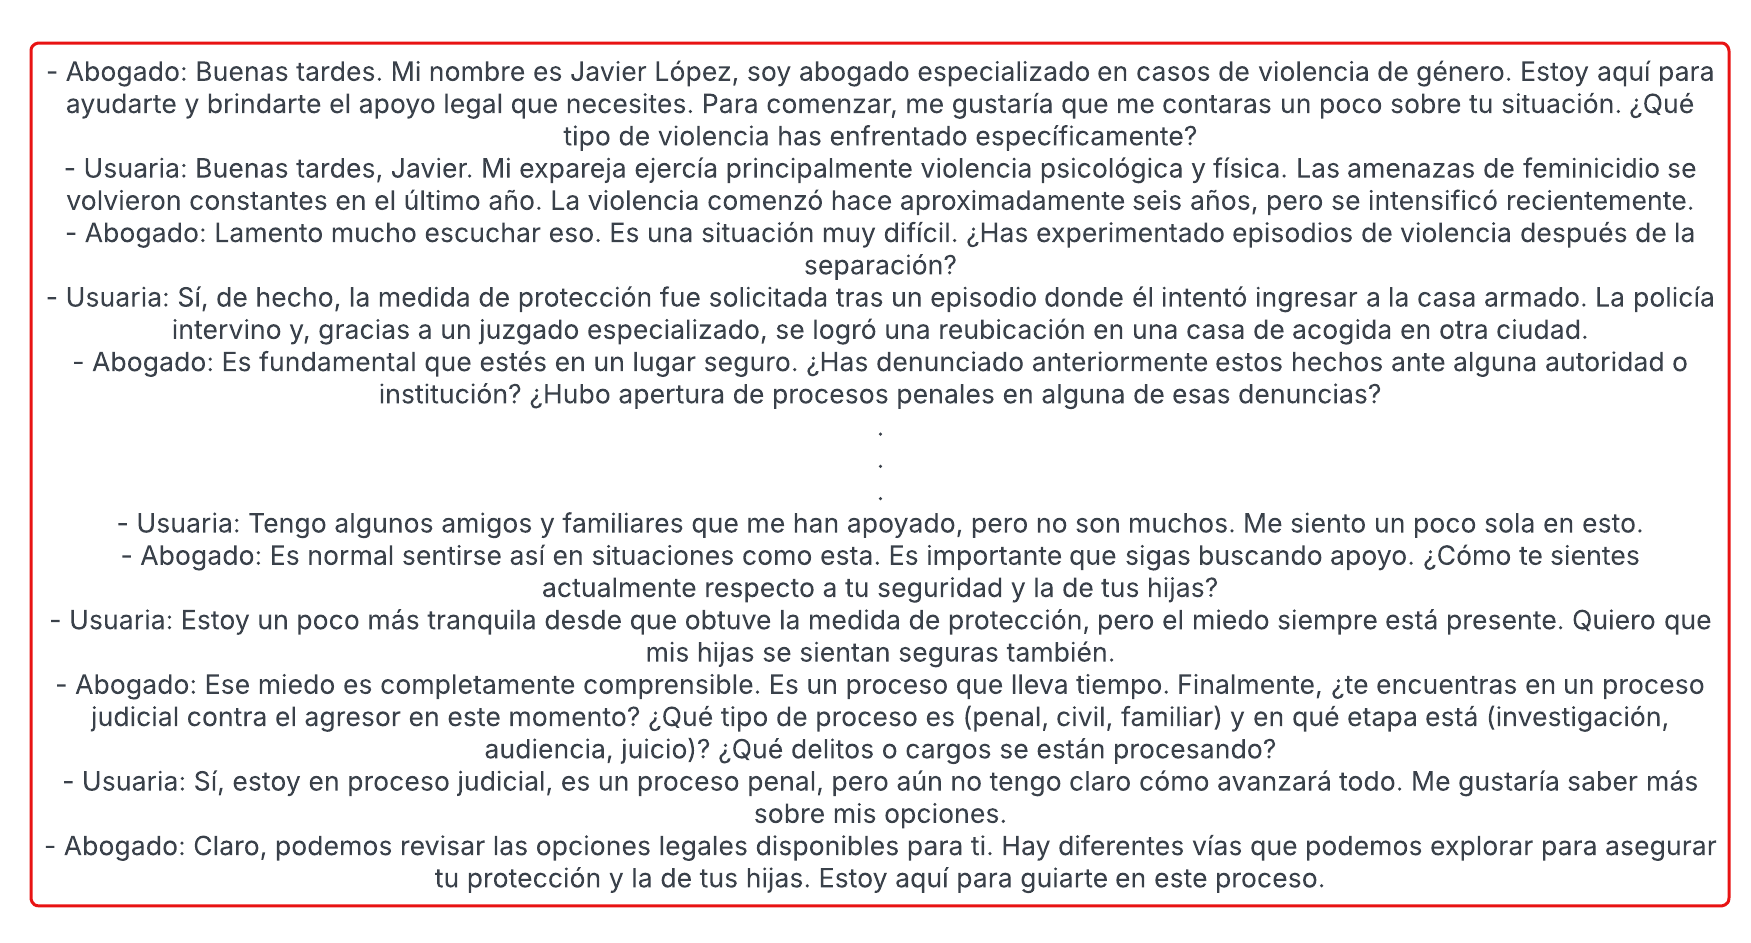
\includegraphics[width=0.7\textwidth]{figures/corrected_conversation.png}
    \caption{Corrected conversation}
    \label{fig:corrected_conversation}
\end{figure}

\begin{figure}[htbp]
    \centering
    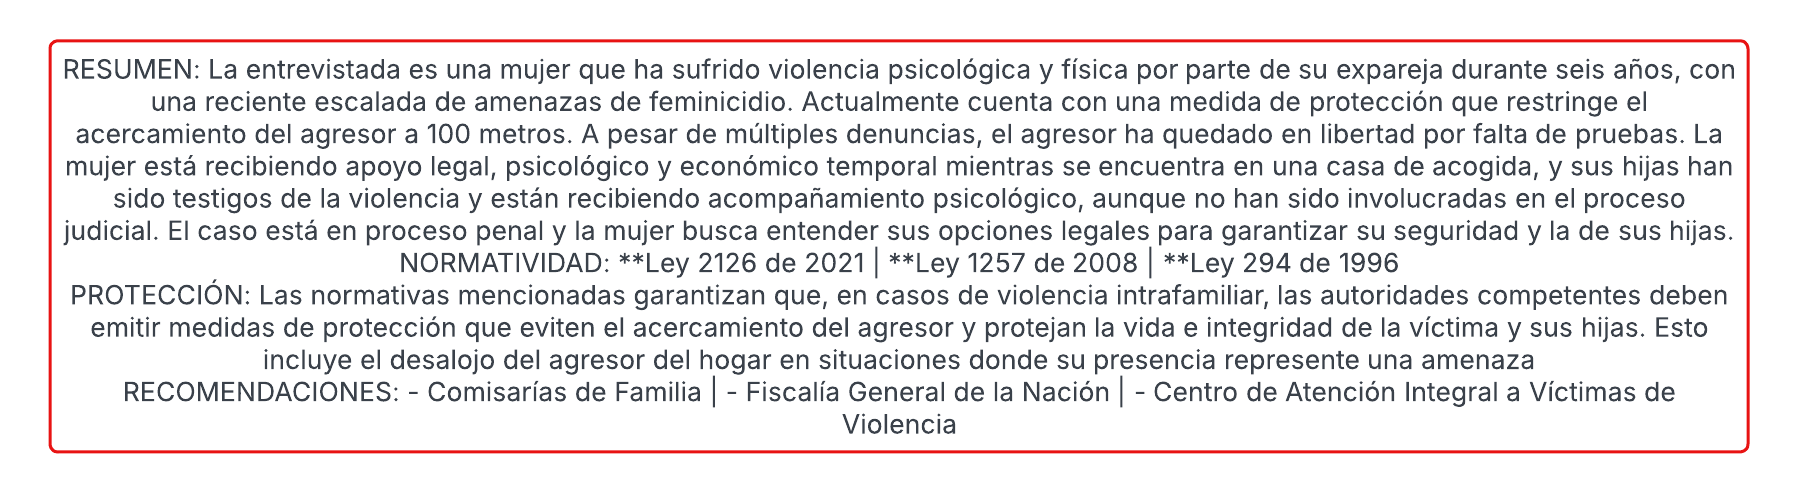
\includegraphics[width=0.7\textwidth]{figures/output_summary.png}
    \caption{Example of a case summary and legal strategy}
    \label{fig:output_summary}
\end{figure}

\section{Agentic Pipeline Development}
\subsection{System Architecture}
\label{sec:architecture}

Our agentic pipeline employs a three-stage architecture for legal case processing, 
as shown in Figure~\ref{fig:chatbot_architecture}. 
Each component operates sequentially with checks between stages.

\begin{figure}[htbp]
    \centering
    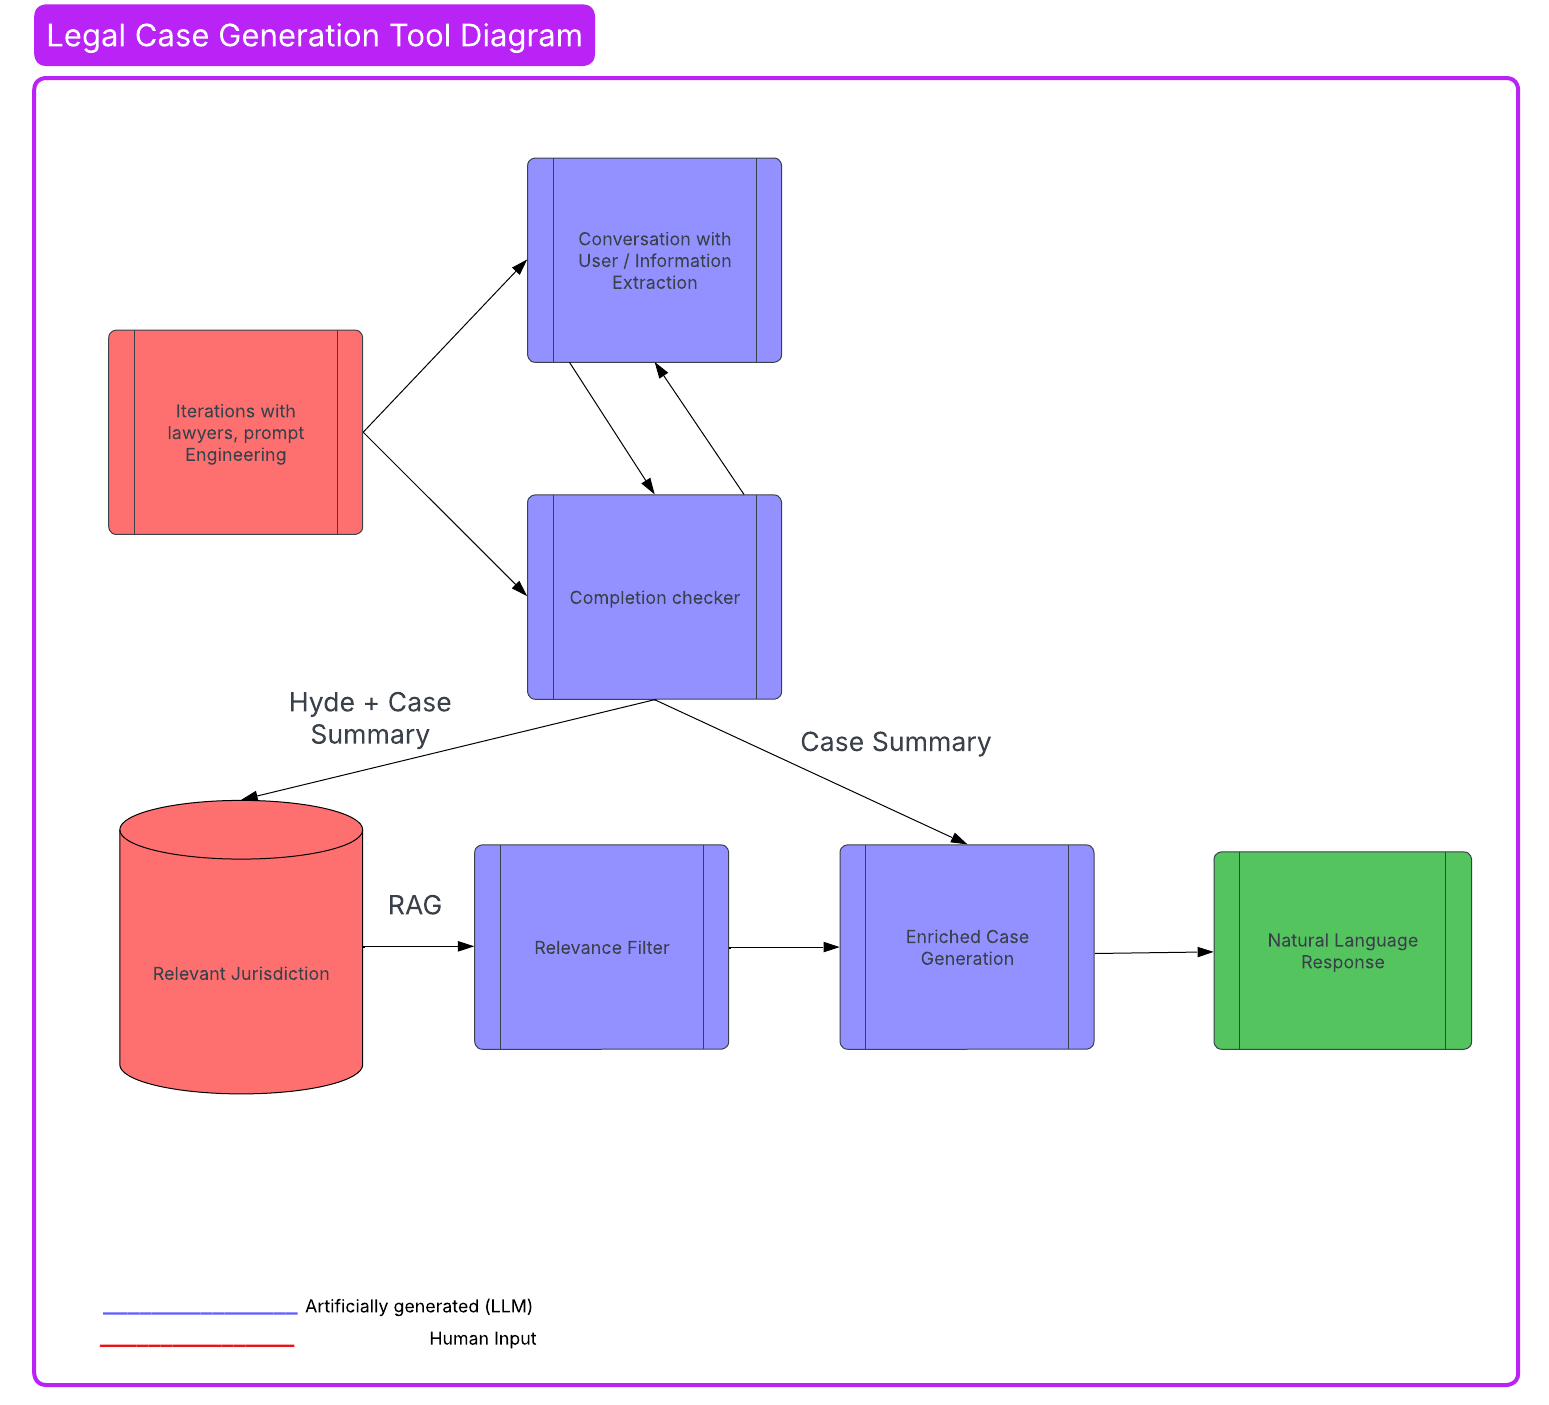
\includegraphics[width=0.7\textwidth]{figures/Chatbot_arch.png}
    \caption{Chatbot Architecture}
    \label{fig:chatbot_architecture}
\end{figure}

\subsection{Information Extraction Module}
The Information Extraction Module is responsible for conducting the initial legal interview with the user. 
Acting as a virtual lawyer, the assistant guides the user through a series of structured questions to collect 
all relevant information about their case, such as the type of violence, the sequence of events, available evidence, 
and the user's objectives. Throughout the conversation, the system manages the state of the interview, keeping track of 
the questions asked, the information gathered, and the user's location within Colombia. The system uses the Legal Interview Prompt 
(see Appendix~\ref{app:prompts}, Section~\ref{sec:legal-interview-prompts}, Subsection~\ref{subsec:legal-interview-prompt}) 
to establish the conversational flow. Due to OpenAI's content safety filters, 
we also preprocess input to handle sensitive content appropriately; this was a particularly difficult task due to the nature 
of the cases and is explored further later. 
After each exchange, the module checks whether enough information has been collected to proceed 
(using the Completion Checker Prompt in Appendix~\ref{app:prompts}, Section~\ref{sec:legal-interview-prompts}, 
Subsection~\ref{subsec:completion-checker-prompt}), either by reaching a predefined threshold or 
by signals from the user or assistant.
\subsubsection{Sensitive Content Handling}
To ensure that conversations could address sensitive topics without being interrupted by content safety filters, 
we implemented a preprocessing step for user input. This was necessary because OpenAI's content moderation system 
can block or flag messages containing explicit or potentially triggering language, which is common in legal cases 
involving violence or abuse. Through some iterations with legal experts, we identified recurring patterns and terms 
that tended to trigger these filters. The function developed for this purpose uses both a dictionary of direct replacements 
and a set of regular expressions to sanitize sensitive content, including sexual, economic, 
physical, and psychological abuse. This preprocessing allows the conversation to remain fluid and focused on the legal issues, 
even when discussing difficult subjects.

\subsection{Legal Case Generation}
The Legal Case Generation module takes the information collected during the interview and organizes it into a structured legal case summary. 
This process involves filtering the conversation data to extract key details, such as the parties involved, the classification of the case, 
a timeline of events, a list of evidence, and the client's main concerns or requests. The module ensures that all relevant facts are included 
and that the information is presented in a format suitable for legal analysis. This structured summary serves as the input for retrieving 
applicable legal documents and generating tailored legal guidance in the subsequent stages.

\subsection{Legal Strategy Generation}
Once the case summary is complete, the system uses a Retrieval-Augmented Generation (RAG) approach to provide legal guidance. 
First, it generates a hypothetical legal document using the HyDE technique 
(see Appendix~\ref{app:prompts}, Section~\ref{sec:legal-interview-prompts}, Subsection~\ref{subsec:hyde-prompt}), 
based on the details of the user's case. The system then searches a 
FAISS vector database containing over 2,000 Colombian legal documents across multiple jurisdictions, including Departamental, Nacional, and 
General categories.

The document database was preprocessed and segmented, with a total of 2,057 individual segments created from the original legal texts. 
Each document was split based on legal hierarchical markers (such as LEY, CAPÍTULO, ARTÍCULO) and labeled with detailed metadata including 
jurisdiction, document name, and specific legal references. This preprocessing enables granular retrieval and contextual matching of legal 
provisions to user cases.

During the retrieval process, the system filters results according to the user's department 
(using the Departamento Extraction Prompt in Appendix~\ref{app:prompts}, Section~\ref{sec:legal-interview-prompts}, 
Subsection~\ref{subsec:departamento-prompt}), int his way, both national and local laws are considered. 
The retrieved legal texts are then incorporated into the final case summary 
(using the RAG Summarizer Prompt in Appendix~\ref{app:prompts}, Section~\ref{sec:legal-interview-prompts}, 
Subsection~\ref{subsec:rag-summarizer-prompt}).

\section{Application Development}

\subsection{Web Application Interface: Initial Prototype}
\label{sec:web-interface}

As part of our development process, we created an initial prototype using Streamlit to test the core functionalities of our legal 
assistance system. This early implementation in served as a proof-of-concept rather than a user-ready solution, 
running entirely on local machines which limited its shareability and accessibility.

\begin{figure}[htbp]
    \centering
    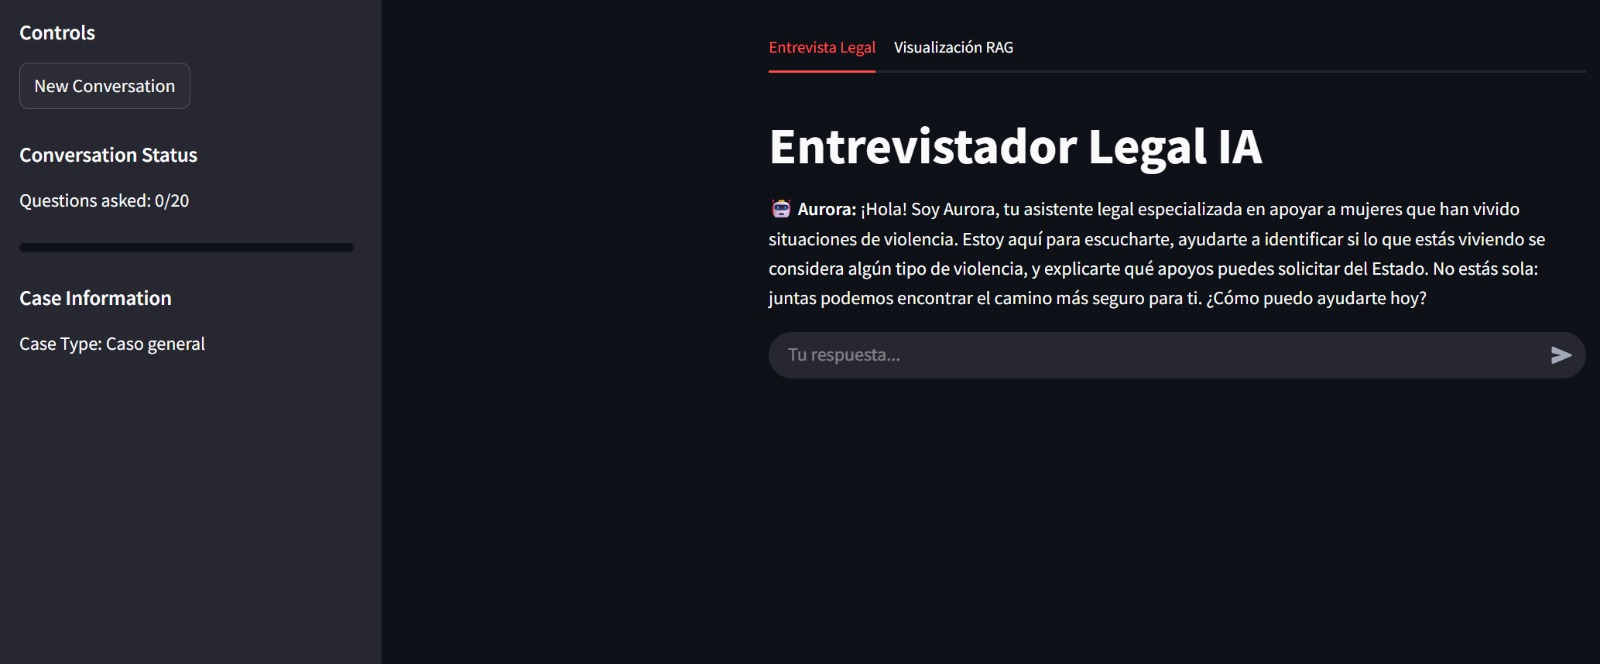
\includegraphics[width=0.7\textwidth]{figures/streamlit.jpeg}
    \caption{Streamlit Interface}
    \label{fig:streamlit}
\end{figure}

\subsubsection{Prototype Interface}
The prototype featured a straightforward interface. 
The Legal Interview section provided a basic chat interface where users could interact with "Aurora". \ref{fig:streamlit}

When a case was completed, the prototype would display a simple success message and the final case summary.

\subsubsection{Technical Limitations}

%This initial prototype faced some technical constraints:
%The application ran exclusively on local development machines, requiring users to have Python and all dependencies installed. 
%This severely limited its shareability and made it impractical for any real-world testing with legal professionals or users.
While deployment was technically possible, it would have significantly limited our customization options. Besides, 
given that the end goal was to create a fully-featured application, developing a proper API architecture
would ultimately provide much greater reliability and flexibility than the Streamlit-based approach.
The interface relied on Streamlit's session state for managing conversation history, which occasionally led to state management 
issues during longer interactions. Message format conversion between the UI and the underlying LangChain components was handled 
through direct manipulation of data structures.

While the prototype implemented the sensitive content preprocessing to avoid content filter issues, 
this solution was not tested. Document rendering was functional but basic, 
with limited formatting options for the legal texts.

\subsubsection{Learning from the Prototype}

Despite its limitations, the initial Streamlit prototype was valuable in revealing insights that would inform later development:
The need for a cloud-based deployment that wouldn't require users to run code locally became evident immediately.

The prototype also demonstrated that while Streamlit was excellent for rapid prototyping, a more robust framework would be needed for a user-ready 
application with better performance and customization options.

This early implementation represented an important step in our development process, allowing us to test functionalities and gather 
feedback that would shape the versions that followed.

\subsection{User Web Application Development}
\label{subsec:web-application}

Following the insights gained from our initial Streamlit prototype, we developed a web application architecture that addressed the limitations of the prototype and enabled broader customization and easier deployment.

%\begin{figure}[htbp]
%    \centering
%    \includegraphics[width=0.8\textwidth]{figures/webapp_architecture.png}
%    \caption{Web Application Architecture}
%    \label{fig:webapp_architecture}
%\end{figure}

\subsubsection{FastAPI Backend Service}

The backend of our production system was implemented using FastAPI, a web framework for building APIs with Python. 
This choice offered many advantages over the Streamlit prototype:
The backend service provided a set of REST endpoints for conversation management, including initializing conversations, sending and receiving messages, 
retrieving case summaries, and accessing RAG documents. This API-centric approach decoupled the Frontend from the underlying AI logic, allowing for multiple client 
applications to connect to the same backend service.

To solve the state management issues encountered in the prototype, we implemented MongoDB integration for conversation persistence. This allowed the system to store 
conversation states, legal contexts, and retrieved documents, enabling long-term storage of user interactions.

The backend handled the complete conversation life-cycle, processing user messages through the legal interview model, 
detecting when cases were completed, triggering the RAG system to retrieve relevant legal documents, and managing the transition 
between conversation and legal summary generation.

We refined the Colombian location detection capabilities to provide more region-specific legal information, implementing detection of Colombian departments in user messages. 
The system also included error handling and logging to diagnose and troubleshoot issues.

\subsubsection{Web Client Implementation}

To make the application accessible to a wide range of users, we developed a lightweight frontend interface:
The frontend was implemented as a static web application using JavaScript and HTML, delivered through a minimal Node.js server. This approach resulted in a design that works across different devices and screen sizes, making the legal assistant accessible from desktop computers, tablets, or mobile phones.

The interface was designed for simplicity and usability, focusing on the conversational interaction with the AI assistant. 
When legal information was retrieved, it was presented along the summary. \ref{fig:Frontend}

The frontend communicated with the backend exclusively through the REST API, allowing for a clean separation of concerns between 
the user interface and the backend processing logic.

\begin{figure}[htbp]
    \centering
    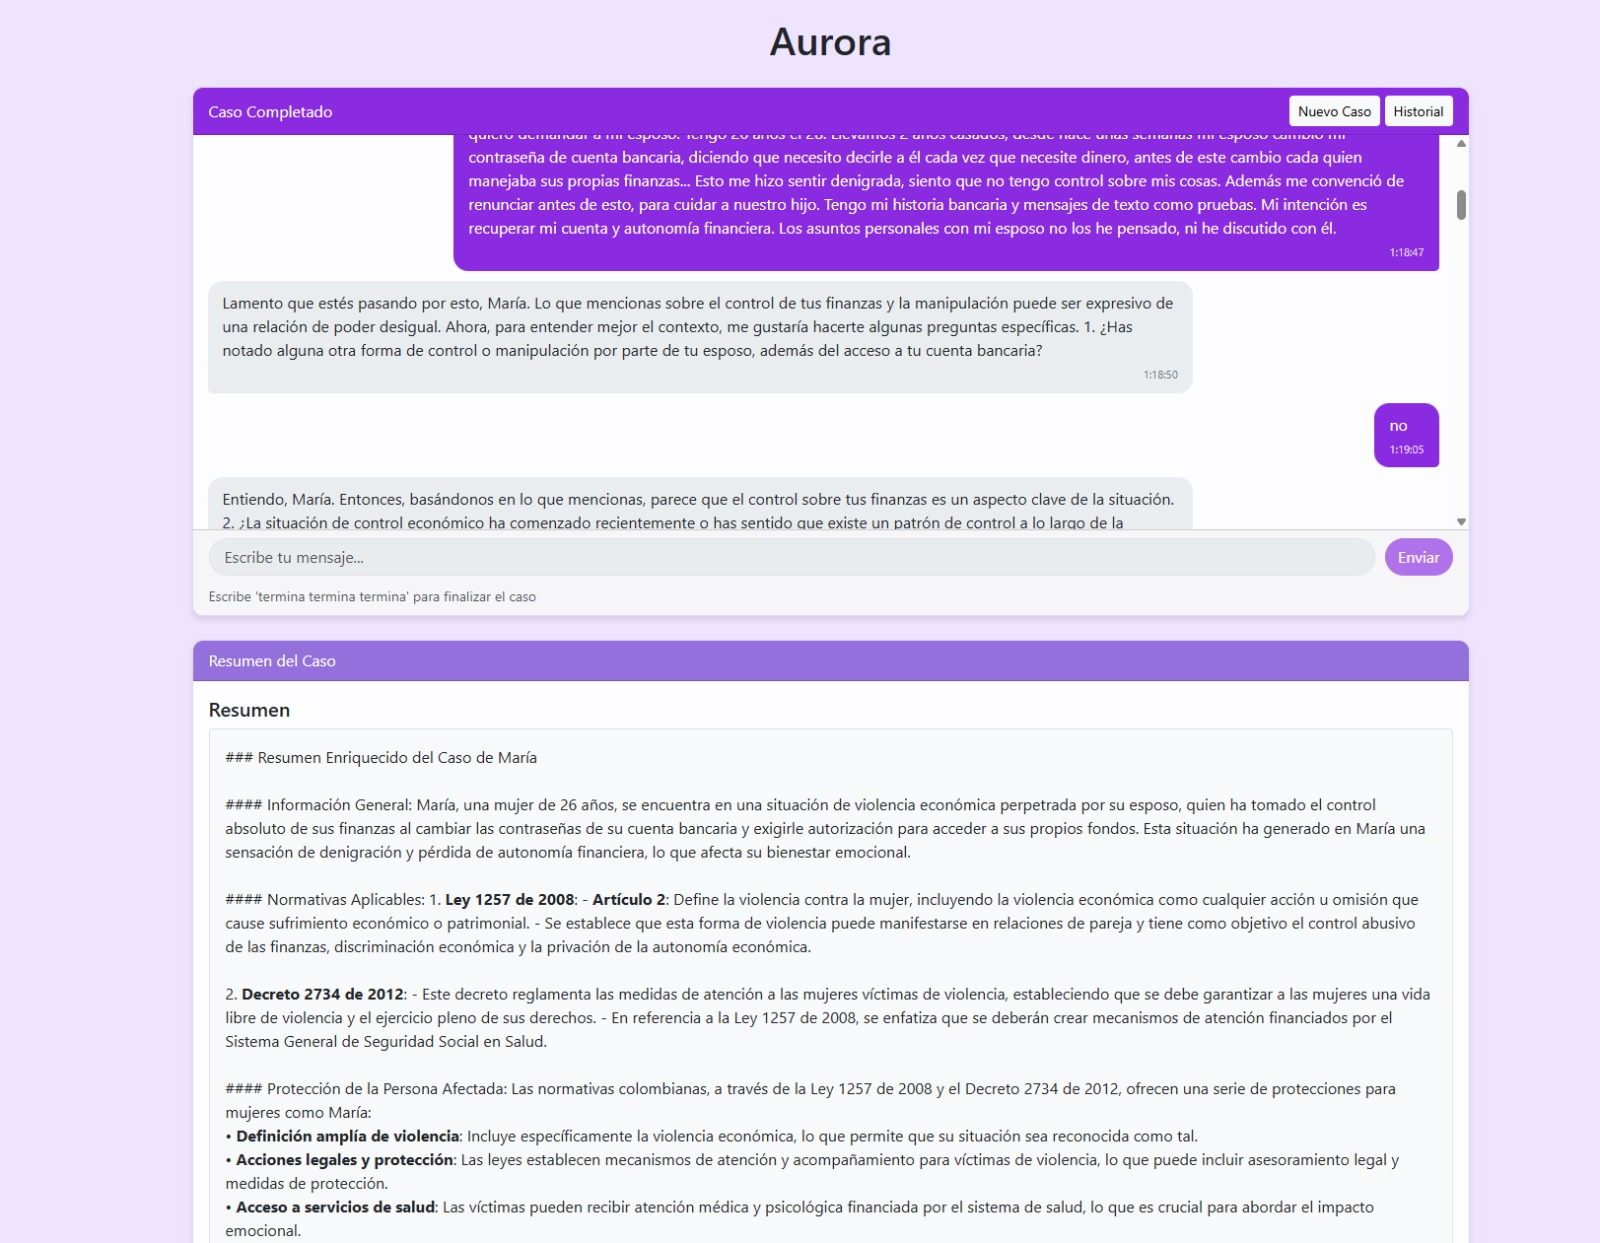
\includegraphics[width=0.8\textwidth]{figures/Frontend.jpeg}
    \caption{Web Application UI}
    \label{fig:Frontend}
\end{figure}

\subsubsection{Containerization and Cloud Deployment}

To facilitate deployment and ensure consistency across environments, the entire application was containerized using Docker:

The containerization process included packaging all required components: the FAISS index for document retrieval, preprocessed legal documents, 
and model code, so that the application had access to all necessary resources regardless of the deployment environment.
For deployment, we developed an automated script that orchestrated the deployment of both backend and frontend components to Google Cloud Run. 

The cloud deployment strategy enabled global accessibility while maintaining reasonable costs, as Cloud Run's serverless architecture only incurred charges when the 
application was actively being used.

\subsection{Initial User Testing}
\label{subsec:user-testing}

To assess the effectiveness of our web application, we conducted limited user testing with a small group of participants including law students, legal professionals, 
and individuals without legal backgrounds. This testing was designed to find the most common issues and improve the system in a very empirical way.

The testing process involved participants engaging with the assistant covering different types of gender-based legal cases as they wished. After each interaction, 
these participants provided feedback on the ease of use, clarity of information, and perceived helpfulness of the legal guidance provided.

This feedback was valuable in understanding both the strengths and limitations of our approach. The positive reception of the conversational interface validated our design 
decisions, while the critiques revealed issues requiring attention.

A significant problem identified during testing was that the RAG system was not behaving optimally. It frequently recommended legal documents that were not applicable to the 
user's specific situation, particularly when regional or departmental legislation was involved. This discovery led us to develop the departamento extraction feature, 
which enabled the system to specifically ask users about their location in Colombia and then filter out non-applicable legislation. This targeted approach  
improved the relevance of the document retrieval process, as users wouldn't receive guidance that was not applicable to them given their geographic location.

Additionally, the testing highlighted the importance of the assistant's tone and communication style. Lawyers from the Consultorio Jurídico emphasized that legal assistants 
in gender-based cases must be especially empathetic and supportive, as clients are often in vulnerable situations. Based on this input, we significantly refined the system's 
prompts to ensure a friendly, supportive, and non-judgmental approach while still maintaining professional boundaries and accuracy.

\subsection{Iterative Prompt Engineering}
\label{subsec:prompt-engineering}

Throughout the development process, an important aspect of our methodology was the iterative refinement of system prompts in close collaboration with legal professionals. 
The prompts detailed in Appendix~\ref{app:prompts} were not static instructions created at the outset of the project, but rather evolved significantly through  
feedback cycles with practicing lawyers and legal scholars. 

The information gathering process itself was structured based on direct input from lawyers at the Consultorio Jurídico. They provided detailed guidance on the specific types of 
information needed to properly assess and address gender-based legal cases in Colombia. This included the appropriate questions, critical data points to collect 
(such as relationship to the aggressor, types of violence experienced, and available evidence), and how to approach sensitive topics in a trauma-informed manner.

This collaborative prompt engineering process involved review sessions where legal experts would interact with the tool, check its legal summaries, and produced document 
retrievals. Their feedback guided substantial revisions to prompt wording, structure, and content focus.

%The iterative prompt engineering process highlights the importance of interdisciplinary collaboration in developing AI systems for specialized domains. 
%While large language models provide powerful capabilities, harnessing these capabilities for domain-specific applications requires ongoing dialogue between 
%technical developers and subject matter experts. The final prompts represent a synthesis of computational and legal knowledge.